\chapter{空气环绕着我们}\label{ch:g2:air-around-us}

在脸前快速挥一挥手：有种柔软的东西
拂过你的脸颊。你看不见它，抓不住它，也没法把它放进抽屉——
可它却充满了每一个房间、每一个瓶子，还有地球上的每一座操场。
本章讲的是\omterm{def:g2:air-around-us:air}{空气}：我们就生活在这层看不见的物质的底部。

\section{空气真的是一种东西吗？}

\begin{definition}[空气]\label{def:g2:air-around-us:air}
\emph{空气}\index{空气}是包围着我们的、看不见的物质。
它没有颜色，没有自身的气味，光能直接穿过它，
这正是我们常常忘记它存在的原因。但它是真实的物质，本章的实验将证明这一点，
而且它非常宝贵：
你每一次呼吸，吸进的都是它。
\end{definition}

\begin{example}[试一试：捉住一些空气]\label{ex:g2:air-around-us:catch}
把一只塑料袋大大张开，在房间里挥一挥，
然后扎紧袋口。袋子鼓得像个小垫子——用手一捏，它会推回来！
里面肯定有东西被关在了里面。打开一个角，再捏一次，
你会感觉到这个看不见的“囚徒”从指缝间溜出来。
一个什么都没有的“空”袋子，是不可能推回来的。
\end{example}

\begin{example}[空气显露自己]\label{ex:g2:air-around-us:shows}
\omterm{def:g2:air-around-us:air}{空气}是看不见的，但它的“把戏”却看得见：热路面上方的\omterm{def:g2:air-around-us:air}{空气}会晃动，
它能托起风筝，吹得树叶沙沙作响，
在水下，只要\omterm{def:g2:air-around-us:air}{空气}逸出，就会冒出气泡。用吸管对着杯中的水吹气，
每一个银色的气泡，
都是一小包正在向上飘的\omterm{def:g2:air-around-us:air}{空气}。
\end{example}

\section{空气占据空间}

\begin{method}[干纸巾潜水]\label{met:g2:air-around-us:drytowel}
这是一个纯粹靠物理原理的小魔术——请在水盆上方进行。
\begin{enumerate}
  \item 把一张干纸巾紧紧地塞进杯底，
        使它不会掉出来；
  \item 把杯子完全倒过来；
  \item 把杯子笔直地压进水盆，水要比整个杯子还深，
        且不能倾斜；
  \item 把杯子笔直地拿出来，摸一摸纸巾。
\end{enumerate}
纸巾完全是干的！这个杯子从来不是空的：它里面充满了\omterm{def:g2:air-around-us:air}{空气}，
被困住的\omterm{def:g2:air-around-us:air}{空气}占着自己的位置，所以水
进不来。
\end{method}

\begin{omfigure}
\begin{tikzpicture}[scale=0.85]
  % basin of water
  \draw[thick] (0,3.2) -- (0,0) -- (9.0,0) -- (9.0,3.2);
  \fill[omDef, opacity=0.15] (0,0) rectangle (9.0,2.7);
  \draw[omDef, thick] (0,2.7) -- (9.0,2.7);
  % the upside-down glass, pushed fully under
  \fill[white] (2.75,0.42) rectangle (4.45,2.28);
  \fill[omDef, opacity=0.15] (2.75,0.42) rectangle (4.45,0.85);
  \draw[line width=2.4pt, omExo!75]
    (2.7,0.4) -- (2.7,2.3) -- (4.5,2.3) -- (4.5,0.4);
  \draw[omDef, thick] (2.75,0.85) -- (4.45,0.85);
  \draw[thick, fill=omMeth, fill opacity=0.5]
    (2.95,1.75) rectangle (4.25,2.15);
  \node[font=\footnotesize, align=center] at (3.6,1.4)
    {被困住的 \\空气};
  % leaders to labels in the open
  \draw[omExo!80, thin] (4.28,1.98) -- (5.4,3.62);
  \node[right, font=\small] at (5.45,3.62) {纸巾，完全是干的};
  \draw[omExo!80, thin] (4.45,0.85) -- (5.8,-0.42);
  \node[right, font=\small] at (5.85,-0.42)
    {水到此为止：空气占着自己的位置};
\end{tikzpicture}

{\small 干纸巾潜水：倒扣的杯子里充满了\omterm{def:g2:air-around-us:air}{空气}，而
两样东西不能同时占据同一个位置。}
\end{omfigure}

\begin{example}[咕噜咕噜的瓶子]\label{ex:g2:air-around-us:glug}
把一只“空”瓶子瓶口朝下压进水盆，再稍稍倾斜：
咕噜，咕噜，咕噜——一个个大大的银色气泡冲向水面，
水则进入瓶中，占据了它们的位置。瓶子里充满了\omterm{def:g2:air-around-us:air}{空气}；
水只能和\omterm{def:g2:air-around-us:air}{空气}一样快地进入，\omterm{def:g2:air-around-us:air}{空气}出得多快，水就进得多快。
厨房水槽里的那一声“咕噜”，
正是\omterm{def:g2:air-around-us:air}{空气}和水在互换位置的声音。
\end{example}

\begin{omfigure}
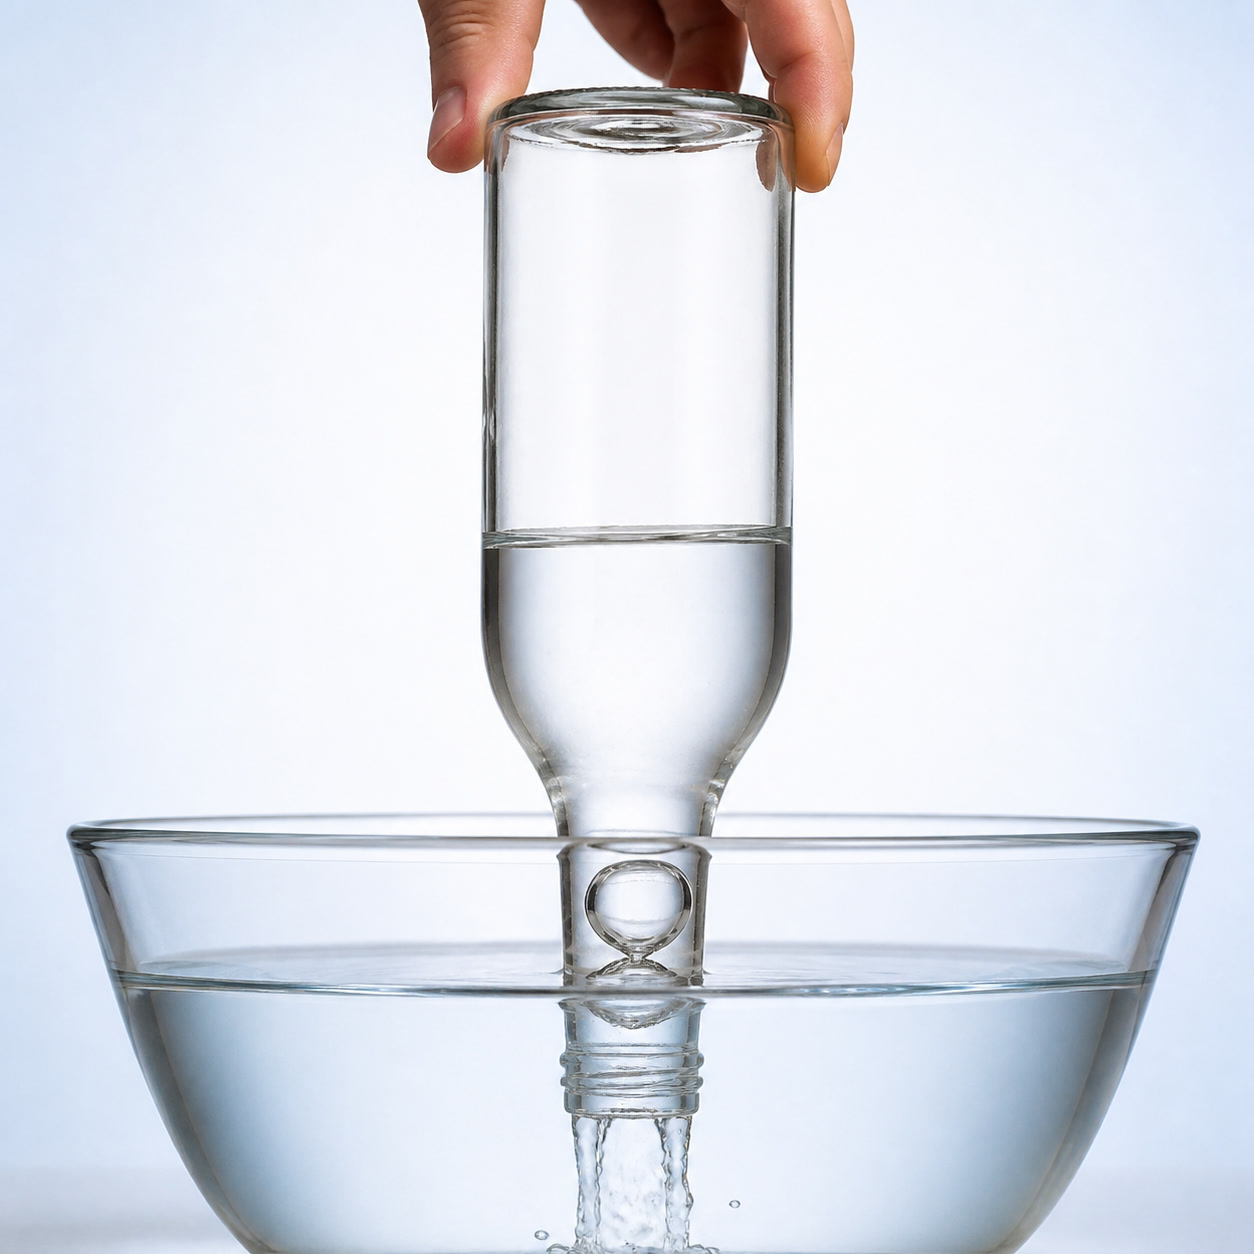
\includegraphics[width=0.42\linewidth]{images/book1/ai/g2-air-glugging-bottle.jpg}

{\small 咕噜咕噜的瓶子：水流出时，大大的\omterm{def:g2:air-around-us:air}{空气}气泡挤着冲进来——瓶中的“空”位置必须被填满。}
\end{omfigure}

\begin{remark}[没有真正空的瓶子]\label{rem:g2:air-around-us:noempty}
从现在起，对“空”这个字要保持怀疑。空瓶子、
空杯子、空盒子，里面全都装满了\omterm{def:g2:air-around-us:air}{空气}，
一直装到边缘。真正的空——里面什么都没有，连\omterm{def:g2:air-around-us:air}{空气}也没有——
是很难做到的，将来有一天，你会遇到科学家给它起的
奇特名字。
\end{remark}

\section{空气会推动物体}

\begin{definition}[风]\label{def:g2:air-around-us:wind}
\emph{风}\index{风}就是流动的\omterm{def:g2:air-around-us:air}{空气}。静止的\omterm{def:g2:air-around-us:air}{空气}碰不到任何人；
而流动的\omterm{def:g2:air-around-us:air}{空气}会推动挡在它路上的任何东西——微风吹拂时轻轻推动，
暴风雨中则强劲到能把树吹弯。
\end{definition}

\begin{example}[空气的工作]\label{ex:g2:air-around-us:work}
流动的\omterm{def:g2:air-around-us:air}{空气}确实能干活：它能把船帆鼓满，让风车玩具转动，
把衣服吹干，还能托起风筝。你自己也会制造风：
每次吹灭生日蜡烛时，你其实都在制造风——
你的呼气是一阵小小的私人风，足以把火苗直接吹离烛芯。
\end{example}

\begin{example}[试一试：气球喷射]\label{ex:g2:air-around-us:balloon}
吹起一个气球，并把它的口捏紧。气球里面，被挤压的\omterm{def:g2:air-around-us:air}{空气}
正等待着。松手后，\omterm{def:g2:air-around-us:air}{空气}向后冲出，
气球便向房间另一头猛地射去，左右晃动得厉害。逃逸的\omterm{def:g2:air-around-us:air}{空气}
推动着气球——这与被挤出的气体推动真正火箭的道理相似，
只是小得多。
\end{example}

\begin{omfigure}
\begin{tikzpicture}[scale=0.85]
  % balloon body and its open neck
  \draw[thick, fill=omThm, fill opacity=0.3]
    (4.75,1.3) ellipse (1.4 and 0.95);
  \draw[thick, fill=omThm, fill opacity=0.3]
    (3.44,1.55) .. controls (3.2,1.48) .. (3.02,1.52)
    -- (3.02,1.08) .. controls (3.2,1.12) .. (3.44,1.05) -- cycle;
  % escaping air, fanning backward
  \draw[-Stealth, omDef, thick] (2.85,1.48) -- (1.65,1.66);
  \draw[-Stealth, omDef, thick] (2.85,1.3) -- (1.55,1.3);
  \draw[-Stealth, omDef, thick] (2.85,1.12) -- (1.65,0.94);
  \node[below, font=\small, omDef] at (1.85,0.66) {空气向后冲出};
  % the flight
  \draw[-Stealth, very thick, omThm] (6.4,1.3) -- (8.1,1.3);
  \node[below right, font=\small, omThm] at (6.3,1.05)
    {气球向前射出};
\end{tikzpicture}

{\small 气球喷射：\omterm{def:g2:air-around-us:air}{空气}向一侧逸出，推动气球向相反方向
运动。}
\end{omfigure}

\begin{remark}[空气很宝贵]\label{rem:g2:air-around-us:breathe}
最重要的“推动”其实悄悄发生在你的胸腔里：每一次
呼吸，\omterm{def:g2:air-around-us:air}{空气}流入，身体留下它需要的一部分，
其余的则流出。人、猫、鸟，甚至鱼（它们靠吸取水中
隐藏的\omterm{def:g2:air-around-us:air}{空气}来呼吸）都需要自己的那一份。看不见
并不等于不重要——对\omterm{def:g2:air-around-us:air}{空气}来说，恰恰相反。
\end{remark}

\section{练习}

\begin{exercise}[$\star$]\label{exo:g2:air-around-us:1}
说出三个你本周见到的、能证明\omterm{def:g2:air-around-us:air}{空气}存在的线索，
且不要用书中的任何实验。
\end{exercise}

\begin{exercise}[$\star$]\label{exo:g2:air-around-us:2}
为什么\cref{ex:g2:air-around-us:catch}中扭紧的袋子
被你一捏就会向回顶？里面装的是什么？
\end{exercise}

\begin{exercise}[$\star$]\label{exo:g2:air-around-us:3}
在“干毛巾潜水”实验中，为什么水没有浸湿毛巾？请用本章的词语说明：
是什么一直占着那个空间？
\end{exercise}

\begin{exercise}[$\star$]\label{exo:g2:air-around-us:4}
在“干毛巾潜水”中，你必须\emph{不}对玻璃杯做什么？
如果你做了，毛巾会怎样？
\end{exercise}

\begin{exercise}[$\star$]\label{exo:g2:air-around-us:5}
瓶子在水下装水时发出的“咕嘟咕嘟”声是怎么回事？什么东西出去了，
什么东西进来了？为什么它们必须轮流进行？
\end{exercise}

\begin{exercise}[$\star$]\label{exo:g2:air-around-us:6}
“请把空瓶子递给我。”空瓶子里
实际上装着什么？（见\cref{rem:g2:air-around-us:noempty}）
\end{exercise}

\begin{exercise}[$\star$]\label{exo:g2:air-around-us:7}
依据\cref{def:g2:air-around-us:wind}中的定义，风是什么？请举出
流动的\omterm{def:g2:air-around-us:air}{空气}所做的两项工作。
\end{exercise}

\begin{exercise}[$\star$]\label{exo:g2:air-around-us:8}
气球喷射飞行时，\omterm{def:g2:air-around-us:air}{空气}向哪个方向冲出，
气球又向哪个方向运动？
\end{exercise}

\begin{exercise}[$\star\star$]\label{exo:g2:air-around-us:9}
一个漏斗紧紧嵌在瓶口里，四周
用粘性橡皮泥密封得严严实实。安娜往漏斗里倒水——
水只咕嘟了一下，便停在漏斗里，不肯
流入瓶中。请解释是什么在阻挡，并提出
一个只需一秒钟的解决办法。
\end{exercise}

\begin{exercise}[$\star\star$]\label{exo:g2:air-around-us:10}
在浴缸的水下，把一只装满\omterm{def:g2:air-around-us:air}{空气}的杯子倒过来，使杯口朝向
另一只同样在水下、装满水的杯子。你能把\omterm{def:g2:air-around-us:air}{空气}
从一只杯子\emph{向上}倒入另一只杯子吗？描述你会看到什么，
以及为什么气泡向上升，而倒出的水却向下流。
\end{exercise}
